%
% Template Laporan Skripsi/Thesis 
%
% @author  Andreas Febrian, Lia Sadita 
% @version 1.03
%
% Dokumen ini dibuat berdasarkan standar IEEE dalam membuat class untuk 
% LaTeX dan konfigurasi LaTeX yang digunakan Fahrurrozi Rahman ketika 
% membuat laporan skripsi. Konfigurasi yang lama telah disesuaikan dengan 
% aturan penulisan thesis yang dikeluarkan UI pada tahun 2008.
%

%
% Tipe dokumen adalah report dengan satu kolom. 
%
\documentclass[12pt, a4paper, onecolumn, oneside, final]{report}

% Load konfigurasi LaTeX untuk tipe laporan thesis
\usepackage{uithesis}
\usepackage{natbib}
\usepackage{import}
% Load konfigurasi khusus untuk laporan yang sedang dibuat
%-----------------------------------------------------------------------------%
% Informasi Mengenai Dokumen
%-----------------------------------------------------------------------------%
% 
% Judul laporan. 
\var{\judul}{Judul Sesuatu Banget \f{English} Miring Juga}
% 
% Tulis kembali judul laporan, kali ini akan diubah menjadi huruf kapital
\Var{\Judul}{JUDUL SESUATU BANGET \f{ENGLISH} MIRING JUGA}
% 
% Tulis kembali judul laporan namun dengan bahasa Ingris
\var{\judulInggris}{Sesuatu Banget in English}

% 
% Tipe laporan, dapat berisi Skripsi, Tugas Akhir, Thesis, atau Disertasi
\var{\type}{Skripsi}
% 
% Tulis kembali tipe laporan, kali ini akan diubah menjadi huruf kapital
\Var{\Type}{Skripsi}
% 
% Tulis nama penulis 
\var{\penulis}{Cicak Bin Kadal}
% 
% Tulis kembali nama penulis, kali ini akan diubah menjadi huruf kapital
\Var{\Penulis}{Cicak Bin Kadal}
% 
% Tulis NPM penulis
\var{\npm}{1234567890}
% 
% Tuliskan Fakultas dimana penulis berada
\Var{\Fakultas}{Ilmu Komputer}
\var{\fakultas}{Ilmu Komputer}
% 
% Tuliskan Program Studi yang diambil penulis
\Var{\Program}{Ilmu Komputer}
\var{\program}{Ilmu Komputer}
\var{\programEng}{Computer Science}
% 
% Tuliskan tahun publikasi laporan
\Var{\bulanTahun}{Juli 2013}
% 
% Tuliskan gelar yang akan diperoleh dengan menyerahkan laporan ini
\var{\gelar}{Sarjana Ilmu Komputer}
% 
% Tuliskan tanggal pengesahan laporan, waktu dimana laporan diserahkan ke 
% penguji/sekretariat
\var{\tanggalPengesahan}{21 Juni 2013} 
% 
% Tuliskan tanggal keputusan sidang dikeluarkan dan penulis dinyatakan 
% lulus/tidak lulus
\var{\tanggalLulus}{5 Juli 2013}
% 
% Tuliskan pembimbing 
\var{\pembimbing}{Prof. Saya }
\var{\pembimbingdua}{Dia S.Kom, M.Kom}
% 
% Alias untuk memudahkan alur penulisan paa saat menulis laporan
\var{\saya}{Penulis}

%-----------------------------------------------------------------------------%
% Judul Setiap Bab
%-----------------------------------------------------------------------------%
% 
% Berikut ada judul-judul setiap bab. 
% Silahkan diubah sesuai dengan kebutuhan. 
% 
\Var{\kataPengantar}{Kata Pengantar}
\Var{\babSatu}{Pendahuluan}
\Var{\babDua}{Landasan Teori}
\Var{\babTiga}{Aplikasi Yang Digunakan}
\Var{\babEmpat}{Perancangan Implementasi dan Analisis}
\Var{\babLima}{Implementasi dan Pengujian}
\Var{\babEnam}{Hasil Implementasi dan Evaluasi}
\Var{\babTujuh}{Kesimpulan dan Saran}

% Daftar pemenggalan suku kata dan istilah dalam LaTeX
%
% Hyphenation untuk Indonesia 
%
% @author  Andreas Febrian
% @version 1.00
% 
% Tambahkan cara pemenggalan kata-kata yang salah dipenggal secara otomatis 
% oleh LaTeX. Jika kata tersebut dapat dipenggal dengan benar, maka tidak 
% perlu ditambahkan dalam berkas ini. Tanda pemenggalan kata menggunakan 
% tanda '-'; contoh:
% menarik
%   --> pemenggalan: me-na-rik
%

\hyphenation{
    % alphabhet A
    a-na-li-sa a-tur 
    a-pli-ka-si 
    % alphabhet B
    ba-ngun-an 
    be-be-ra-pa 
    ber-ge-rak
    ber-ke-lan-jut-an 
    ber-pe-nga-ruh 
    % alphabhet C
    ca-ri
    % alphabhet D
    di-ban-ding-kan
    di-de-fi-ni-si-kan
    di-ha-rap-kan
    di-ka-te-go-ri-kan
    di-mi-li-ki-nya
    di-se-rah-kan
    di-sim-pan di-pim-pin de-ngan da-e-rah di-ba-ngun da-pat di-nya-ta-kan 
    di-sim-bol-kan di-pi-lih di-li-hat de-fi-ni-si
    di-se-su-ai-kan
    % alphabhet E
    e-le-men
    e-ner-gi eks-klu-sif
    % alphabhet F
    fa-si-li-tas
    % alphabhet G
    ga-bung-an ge-rak
    % alphabhet H
    ha-lang-an
    he-te-ro-gen
    % alphabhet I
    i-ngin
    % alphabhet J
    % alphabhet K
    ke-hi-lang-an
    ku-ning 
    kua-li-tas ka-me-ra ke-mung-kin-an ke-se-pa-ham-an
    ke-te-pat-an
    kon-fi-gu-ra-si
    % alphabhet L
    ling-kung-an
    % alphabhet M
    me-min-ta
    me-mo-del-kan
    me-mo-ri
    men-de-fi-ni-si-kan
    me-neng-ah
    meng-a-tas-i me-mung-kin-kan me-nge-na-i me-ngi-rim-kan 
    meng-u-bah meng-a-dap-ta-si me-nya-ta-kan mo-di-fi-ka-si
    meng-a-tur
    meng-au-to-ma-si
    meng-a-ko-mo-da-si
    me-ngo-rek-si
    % alphabhet N
    nya-ta non-eks-klu-sif
    % alphabhet O
    % alphabhet P
    pa-ra-lel
    peng-ala-mat-an
    pen-ting
    penga-da-an
	pe-nye-rap-an 
	pe-ngon-trol
    pe-mo-del-an
    pe-ran  pe-ran-an-nya
    pe-rin-tah
    pem-ba-ngun-an pre-si-den pe-me-rin-tah prio-ri-tas peng-am-bil-an 
    peng-ga-bung-an pe-nga-was-an pe-ngem-bang-an 
    pe-nga-ruh pa-ra-lel-is-me per-hi-tung-an per-ma-sa-lah-an 
    pen-ca-ri-an peng-struk-tur-an
    pe-ner-bang-an
    pro-se-sor
    % alphabhet Q
    % alphabhet R
    ran-cang-an
    % alphabhet S
    se-dang-kan
    se-ring
    si-mu-la-si sa-ngat    
    % alphabhet T
    te-ngah
    ter-da-pat
    % alphabhet U
    u-sa-ha
    % alphabhet V
    % alphabhet W
    % alphabhet X
    % alphabhet Y
    % alphabhet Z
    % special
}
% Daftar istilah yang mungkin perlu ditandai 
%
% @author  Andreas Febrian
% @version 1.00
% 
% Mendaftar seluruh istilah yang mungkin akan perlu dijadikan 
% italic atau bold pada setiap kemunculannya dalam dokumen. 
% 

\var{\license}{\f{Creative Common License 1.0 Generic}}
\var{\bslash}{$\setminus$}


%\usepackage[backend=bibtex]{biblatex}
%\addbibresource{bib.bib}

% Awal bagian penulisan laporan
\begin{document}
%
% Sampul Laporan
%
% Sampul Laporan

%
% @author  unknown
% @version 1.01
% @edit by Andreas Febrian
%

\begin{titlepage}
    \begin{center}    
        \begin{figure}
            \begin{center}
                
\includegraphics[width=2.5cm]{pics/makara.png}
            \end{center}
        \end{figure}    
        \vspace*{0cm}
        \bo{
        	UNIVERSITAS INDONESIA\\
        }
        
        \vspace*{1.0cm}
        % judul thesis harus dalam 14pt Times New Roman
        \bo{\Judul} \\[1.0cm]

        \vspace*{2.5 cm}    
        % harus dalam 14pt Times New Roman
        \bo{\Type}

        \vspace*{3 cm}       
        % penulis dan npm
        \bo{\Penulis} \\
        \bo{\npm} \\

        \vspace*{5.0cm}

        % informasi mengenai fakultas dan program studi
        \bo{
        	FAKULTAS \Fakultas\\
        	PROGRAM STUDI \Program \\
        	DEPOK \\
        	\bulanTahun
        }
    \end{center}
\end{titlepage}


%
% Gunakan penomeran romawi
\pagenumbering{roman}

%
% load halaman judul dalam
\addChapter{HALAMAN JUDUL}
%
% Halaman Judul Laporan 
%
% @author  unknown
% @version 1.01
% @edit by Andreas Febrian
%

\begin{titlepage}
    \begin{center}\begin{figure}
            \begin{center}
                
\includegraphics[width=2.5cm]{pics/makara.png}
            \end{center}
        \end{figure}    
        \vspace*{0cm}
        \bo{
        	UNIVERSITAS INDONESIA\\
        }
        
        \vspace*{1.0cm}
        % judul thesis harus dalam 14pt Times New Roman
        \bo{\Judul} \\[1.0cm]

        \vspace*{2.5 cm}    
        % harus dalam 14pt Times New Roman
        \bo{\Type} \\
        % keterangan prasyarat
        \bo{Diajukan sebagai salah satu syarat untuk memperoleh gelar \\
        \gelar}\\

        \vspace*{3 cm}       
        % penulis dan npm
        \bo{\Penulis} \\
        \bo{\npm} \\

        \vspace*{5.0cm}

        % informasi mengenai fakultas dan program studi
        \bo{
        	FAKULTAS \Fakultas\\
        	PROGRAM STUDI \Program \\
        	DEPOK \\
        	\bulanTahun
        }
    \end{center}
\end{titlepage}

%
% setelah bagian ini, halaman dihitung sebagai halaman ke 2
\setcounter{page}{2}

% sementara ga usah
% load halaman pengesahan
%\addChapter{LEMBAR PERSETUJUAN}
%%
% Halaman Pengesahan
%
% @author  Andreas Febrian
% @author  Ardhi Putra Pratama
% @version 1.1
%

\chapter*{HALAMAN PERSETUJUAN}

\vspace*{0.2cm}
\noindent 

\noindent
\begin{tabular}{l l p{11cm}}
	\bo{Judul}&: & \judul \\ 
	\bo{Nama}&: & \penulis \\
	\bo{NPM}&: & \npm \\
\end{tabular} \\

\vspace*{1.2cm}


\noindent\begin{minipage}[b]{0.6\hsize}
  \raggedright
  Laporan \type~ini telah diperiksa dan disetujui.\\[0.3cm]
  
  \tanggalPengesahan \\[2cm]
  
  \underline{\pembimbing}\\[0.1cm]
  Pembimbing \type
\end{minipage}
\hfill
\begin{minipage}[b]{0.4\hsize}
  \raggedleft
  .\\[2cm]
  \underline{\pembimbingdua}\\[0.1cm]
  Pembimbing \type
\end{minipage}

\newpage
%
% load halaman orisinalitas 
\addChapter{LEMBAR PERNYATAAN ORISINALITAS}
%
% Halaman Orisinalitas
%
% @author  Andreas Febrian
% @version 1.01
%

\chapter*{\uppercase{halaman pernyataan orisinalitas}}
\vspace*{2cm}

\begin{center}
	\bo{\type~ini adalah hasil karya saya sendiri, \\ 
	dan semua sumber baik yang dikutip maupun dirujuk \\
	telah saya nyatakan dengan benar.} \\
	\vspace*{2.6cm}
	
	\begin{tabular}{l c l}
	\bo{Nama} & : & \bo{\penulis} \\
	\bo{NPM} & : & \bo{\npm} \\ 
	\bo{Tanda Tangan} & : & \\
	& & \\
	& & \\
	\bo{Tanggal} & : & \bo{\tanggalPengesahan} \\	
	\end{tabular}
\end{center}

\newpage
%
%
\addChapter{LEMBAR PENGESAHAN}
%
% Halaman Pengesahan Sidang
%
% @author  Andreas Febrian, Andre Tampubolon 
% @version 1.02
%

\chapter*{HALAMAN PENGESAHAN}

\vspace*{0.4cm}
\noindent 

\noindent
\begin{tabular}{ll p{9cm}}
	\type~ini diajukan oleh&: & \\
	Nama&: & \penulis \\
	NPM&: & \npm \\
	Program Studi&: & \program \\
	Judul \type&: & \judul \\
\end{tabular} \\

\vspace*{1.0cm}

\noindent \bo{Telah berhasil dipertahankan di hadapan Dewan Penguji 
dan diterima sebagai bagian persyaratan yang diperlukan untuk 
memperoleh gelar \gelar~pada Program Studi \program, Fakultas 
\fakultas, Universitas Indonesia.}\\[0.2cm]

\begin{center}
	\bo{DEWAN PENGUJI}
\end{center}

\vspace*{0.3cm}

\begin{tabular}{l l l l }
	& & & \\
	Pembimbing&: & \pembimbing & (\hspace*{3.0cm}) \\
	& & & \\
	Pembimbing&: & \pembimbingdua & (\hspace*{3.0cm}) \\
	& & & \\
	Penguji&: & Penguji 1 & (\hspace*{3.0cm}) \\
	& & & \\
	Penguji&: & Penguji 2 & (\hspace*{3.0cm}) \\
\end{tabular}\\

\vspace*{2.0cm}

\begin{tabular}{ll l}
	Ditetapkan di&: & Depok\\
	Tanggal&: & \tanggalLulus \\
\end{tabular}


\newpage
%
%
\addChapter{\kataPengantar}
%-----------------------------------------------------------------------------%
\chapter*{\kataPengantar}
%-----------------------------------------------------------------------------%
\f{Alhamdulillahirabbil'alamin}, segala puji dan syukur kehadirat Tuhan Yang Maha Esa, Allah Subhana Huwataala, karena hanya dengan hidayah dan rahmat-Nya, penulis dapat menyelesaikan pembuatan skripsi ini.

\f{Allahumma sholli 'alaa sayyidina Muhammad}, Sholawat serta salam tak henti-hentinya dipanjatkan kepada Rasulullah SAW, atas peranannya di muka bumi dalam memberikan tuntunan kepada seluruh umat manusia, dan sebagai inspirasi atas seluruh manusia sebagai manusia dengan akhlak terbaik.

Penulisan skripsi ini ditujukan untuk memenuhi salah satu syarat untuk menyelesaikan pendidikan pada Program \gelar, Universitas Indonesia. Saya sadar bahwa dalam perjalanan menempuh kegiatan penerimaan dan adaptasi, belajar-mengajar, hingga penulisan skripsi ini, penulis tidak sendirian. Penulis ingin berterima kasih kepada pihak-pihak berikut : 

\vspace*{0.1cm}
\begin{flushright}
Depok, 17 Juni 2013\\[0.1cm]
\vspace*{1cm}
\penulis

\end{flushright}
%
%
\addChapter{LEMBAR PERSETUJUAN PUBLIKASI ILMIAH}
% 
% @author  Andre Tampubolon, Andreas Febrian
% @version 1.01
% 

\chapter*{\uppercase{Halaman Pernyataan Persetujuan Publikasi Tugas Akhir untuk Kepentingan Akademis}}

\vspace*{0.2cm}
\noindent 
Sebagai sivitas akademik Universitas Indonesia, saya yang bertanda 
tangan di bawah ini:
\vspace*{0.4cm}


\begin{tabular}{p{4.2cm} l p{6cm}}
	\bo{Nama} & : & \penulis \\ 	
	\bo{NPM} & : & \npm \\
	\bo{Program Studi} & : & \program\\	
	\bo{Fakultas} & : & \fakultas\\
	\bo{Jenis Karya} & : & \type \\
\end{tabular}

\vspace*{0.6cm}
\noindent demi pengembangan ilmu pengetahuan, menyetujui untuk memberikan 
kepada Universitas Indonesia \bo{Hak Bebas Royalti Noneksklusif 
(Non-exclusive Royalty Free Right)} atas karya ilmiah saya yang berjudul:
\begin{center}
	\judul
\end{center}
beserta perangkat yang ada (jika diperlukan). Dengan Hak Bebas Royalti 
Noneksklusif ini Universitas Indonesia berhak menyimpan, 
mengalihmedia/formatkan, mengelola dalam bentuk pangkalan data 
(\f{database}), merawat, dan memublikasikan tugas akhir saya selama 
tetap mencantumkan nama saya sebagai penulis/pencipta dan sebagai 
pemilik Hak Cipta. \\

\noindent Demikian pernyatan ini saya buat dengan sebenarnya.

\begin{center}
	\vspace*{0.8cm}
	\begin{tabular}{lll}
		Dibuat di&: & Depok \\
		Pada tanggal&: & \tanggalPengesahan \\
	\end{tabular}\\

	\vspace*{0.2cm}
	Yang menyatakan \\
	\vspace*{2cm}
	(\penulis)
\end{center}

\newpage


%
% 
\singlespacing
\addChapter{ABSTRAK}
%
% Halaman Abstrak
%
% @author  Andreas Febrian
% @version 1.00
%

\chapter*{Abstrak}

\vspace*{0.2cm}

\noindent \begin{tabular}{l l p{10cm}}
	Nama&: & \penulis \\
	Program Studi&: & \program \\
	Judul&: & \judul \\
\end{tabular} \\ 

\vspace*{0.5cm}

\noindent 
\\ Abstrak INA

\vspace*{0.2cm}

\noindent Kata Kunci: \\ 
\noindent satu, dua, \textit{tiga}\\ 

\newpage

%
%
%
% Halaman Abstract
%
% @author  Andreas Febrian
% @version 1.00
%

	\chapter*{ABSTRACT}

\vspace*{0.2cm}

\noindent \begin{tabular}{l l p{11.0cm}}
	Name&: & \penulis \\
	Program&: & \programEng \\
	Title&: & \judulInggris \\
\end{tabular} \\ 

\vspace*{0.5cm}

\noindent 
\\ Abstract in Eng

\vspace*{0.2cm}

\noindent Keywords: \\ 
\noindent one,two,three\\

\newpage

%
% Daftar isi, gambar, dan tabel
%
\tableofcontents
\clearpage
\listoffigures
\clearpage
\listoftables
\clearpage
\lstlistoflistings
\clearpage

%
% Gunakan penomeran Arab (1, 2, 3, ...) setelah bagian ini.
%
\pagenumbering{arabic}

%
%
%
\onehalfspacing
%-----------------------------------------------------------------------------%
\chapter{\babSatu}
%-----------------------------------------------------------------------------%


%-----------------------------------------------------------------------------%
\section{Latar Belakang}
%-----------------------------------------------------------------------------%

Menurut \citeauthor{book.buyya} terdapat 3 buah contoh untuk membuat enumerate pada latex \citep{book.buyya}: 
\begin{enumerate}
\item Makan
\item Minum
\end{enumerate}\paragraph{}

Menurut \cite{ppt.ecmwf}, pemodelan yang sama apabila dijalankan dengan komputer \f{Dual Core} maka akan membutuhkan waktu 1 tahun dengan asumsi memori yang dibutuhkan cukup \citep{ppt.ecmwf}.

%-----------------------------------------------------------------------------%
\section{Perumusan Masalah}
%-----------------------------------------------------------------------------%
Pada bagian ini akan dijelaskan mengenai definisi permasalahan yang dihadapi dan ingin diselesaikan serta asumsi dan batasan yang digunakan dalam menyelesaikannya.

%-----------------------------------------------------------------------------%
\section{Tujuan dan Manfaat Penelitian}
%-----------------------------------------------------------------------------%
Dibawah ini adalah contoh itemize : 
\begin{itemize}
\item Terimplementasinya .
\item Menyelesaikan masalah .
\end{itemize}
\paragraph{}

%-----------------------------------------------------------------------------%
\section{Tahapan Penelitian}
%-----------------------------------------------------------------------------%
\todo{Tuliskan tujuan penelitian.}
%-----------------------------------------------------------------------------%
\section{Ruang Lingkup Penelitian}
%-----------------------------------------------------------------------------%

%-----------------------------------------------------------------------------%
\section{Sistematika Penulisan}
%-----------------------------------------------------------------------------%
Sistematika penulisan laporan adalah sebagai berikut:
\begin{itemize}
	\item Bab 1 \babSatu \\
	\item Bab 2 \babDua \\
	\item Bab 3 \babTiga \\
	\item Bab 4 \babEmpat \\
	\item Bab 5 \babLima \\
	\item Bab 6 \babEnam \\
	\item Bab 7 \babTujuh \\
\end{itemize}

\todo{Tambahkan penjelasan singkat mengenai isi masing-masing bab.}
%-----------------------------------------------------------------------------%
\chapter{\babDua}
%-----------------------------------------------------------------------------%
Bab ini berisi .... Pada sub-bab \ref{cha:kompar} akan dijelaskan dasar-dasar ...
%-----------------------------------------------------------------------------%
\section{X si sesuatu}\label{cha:kompar}
%-----------------------------------------------------------------------------%
Dokumen \latex~sangat mudah, seperti halnya membuat dokumen teks biasa. Ada beberapa perintah yang diawali dengan tanda '\bslash'. Seperti perintah \bslash\bslash~yang digunakan untuk memberi baris baru. 
Perintah tersebut juga sama dengan perintah \bslash newline. Pada bagian ini akan sedikit dijelaskan cara manipulasi teks dan perintah-perintah \latex~yang mungkin akan sering digunakan. 
Jika ingin belajar hal-hal dasar mengenai \latex, silahkan kunjungi: 
\begin{itemize}
	\item \url{http://frodo.elon.edu/tutorial/tutorial/}, atau
	\item \url{http://www.maths.tcd.ie/~dwilkins/LaTeXPrimer/}
\end{itemize}
%-----------------------------------------------------------------------------%
\subsection{Pengertian X}
%-----------------------------------------------------------------------------%
Setiap gambar dapat diberikan caption dan diberikan label. Label dapat digunakan untuk menunjuk gambar tertentu. Jika posisi gambar berubah, maka nomor gambar juga akan diubah secara 
otomatis. Begitu juga dengan seluruh referensi yang menunjuk pada gambar tersebut. 

Contoh sederhana adalah \pic~\ref{fig:exmasalahparalel}. Silahkan lihat code \latex~dengan nama bab2-landasan-teori.tex untuk melihat kode lengkapnya. Harap diingat bahwa caption untuk gambar selalu terletak dibawah gambar. 

Dibawah adda figure, jangn lupa dimention dengan \ref{fig:exmasalahparalel}. 

\begin{figure}
	\centering
	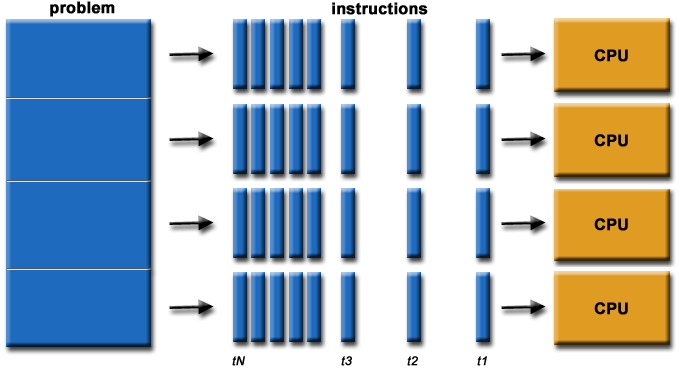
\includegraphics[width=0.8\textwidth]
		{pics/parallelProblem.png}
	\caption{Contoh masalah yang dikerjakan secara paralel}
	\label{fig:exmasalahparalel}
\end{figure}
\vspace{-0.8cm}
\begin{center}
{\small Sumber gambar: \citep{net.oxford}}
\end{center}

%-----------------------------------------------------------------------------%
\subsection{Klasifikasi X}
%-----------------------------------------------------------------------------%
Figure dalam enum dan dua sitasi sekaligus \citep{book.buyya,book.sterling-jones} :  
\begin{enumerate}
\item \bi{Bold Italic} \\
Penjelasan....... Untuk gambarannya dapat dilihat di Gambar \ref{fig:neumann}.

\begin{figure}
	\centering
	\includegraphics[height=0.65\textwidth,width=0.6\textwidth]
		{pics/neumann.pdf}
	\caption{Arsitektur klasik \f{von Neumann}}
	\label{fig:neumann}
\end{figure}
\vspace{-1.2cm}
\begin{center}
{\small Sumber gambar terinspirasi dari: \citep{buku.pressman}}
\end{center} 

\item \bi{Sesuatu banget} \\
Penjelasan.......
\end{enumerate}
\paragraph{}
%-----------------------------------------------------------------------------%
\section{\f{Section in Eng}}
%-----------------------------------------------------------------------------%
Hal pertama yang mungkin ditanyakan adalah bagaimana membuat huruf tercetak tebal, miring, atau memiliki garis bawah. 
Pada Texmaker, Anda bisa melakukan hal ini seperti halnya saat mengubah dokumen dengan LO Writer. 
Namun jika tetap masih tertarik dengan cara lain, ini dia: 

\begin{itemize}
	\item \bo{Bold} \\
		Gunakan perintah \bslash textbf$\lbrace\rbrace$ atau 
		\bslash bo$\lbrace\rbrace$. 
	\item \f{Italic} \\
		Gunakan perintah \bslash textit$\lbrace\rbrace$ atau 
		\bslash f$\lbrace\rbrace$. 
	\item \underline{Underline} \\
		Gunakan perintah \bslash underline$\lbrace\rbrace$.
	\item $\overline{Overline}$ \\
		Gunakan perintah \bslash overline. 
	\item $^{superscript}$ \\
		Gunakan perintah \bslash $\lbrace\rbrace$. 
	\item $_{subscript}$ \\
		Gunakan perintah \bslash \_$\lbrace\rbrace$. 
\end{itemize}

Perintah \bslash f dan \bslash bo hanya dapat digunakan jika package 
uithesis digunakan. 
%-----------------------------------------------------------------------------%
\subsection{Pengertian \f{Section in Eng}}
%-----------------------------------------------------------------------------%

%-----------------------------------------------------------------------------%
\subsection{Next Subsection \f{Section in Eng}}
%-----------------------------------------------------------------------------%

%-----------------------------------------------------------------------------%
\section{\f{Keatas lagi}}
%-----------------------------------------------------------------------------%
Contoh cite yang ga ada \cite{gaib}. Cite author \citeauthor{article.rebecca},cite tahun \citeyear{article.treese}, cite mention \cite{adin.experiment}, dan cite di akhir kalimat \citep{techreport.nist}.
%-----------------------------------------------------------------------------%
\subsection{\f{Masuk lagi}}
%-----------------------------------------------------------------------------%
Footnote example nih : MPICH \footnote{\url{http://www.mpich.org/}}, LAM/MPI \footnote{\url{http://www.lam-mpi.org/}}, dan OpenMPI \footnote{\url{www.open-mpi.org}} \citep{article.mcguire}. MPI-3 sedang dalam tahap perencanaan \footnote{\url{http://meetings.mpi-forum.org/MPI_3.0_main_page.php}}. Fungsi-fungsi tersebut berada di tabel \ref{tab:mpifund}. (Contoh tabel).

\begin{table}
	\centering
	\caption{Fungsi fundamental MPI}
	\label{tab:mpifund}
	\begin{tabular}{|c|c|c|}
	\hline
	\rowcolor{headertbl}	
	\hline No. & Nama Fungsi & Penjelasan \\ 
	\hline 1 & MPI\_Init & Memulai kode MPI \\ 
	\hline 2 & MPI\_Finalize & Mengakhiri kode MPI \\ 
	\hline 3 & MPI\_Comm\_size & Menentukan jumlah proses \\ 
	\hline 4 & MPI\_Comm\_rank & Menentukan label proses \\ 
	\hline 5 & MPI\_Send & Mengirim pesan \\ 
	\hline 6 & MPI\_Recv & Menerima pesan \\ 
	\hline
	\end{tabular}
\end{table}
\begin{center}
{\small Sumber tabel: taro sitasi disini, if i were u}
\end{center}
%-----------------------------------------------------------------------------%
\chapter{\babTiga}
%-----------------------------------------------------------------------------%

%-----------------------------------------------------------------------------%
\section{NPACI Rocks}
%-----------------------------------------------------------------------------%

%-----------------------------------------------------------------------------%
\subsection{XZXX}
%-----------------------------------------------------------------------------%
Ini dapat dilihat di Gambar \ref{fig:alurkickstart} \citep{paper.jackson}. 

\begin{figure}
	\centering
	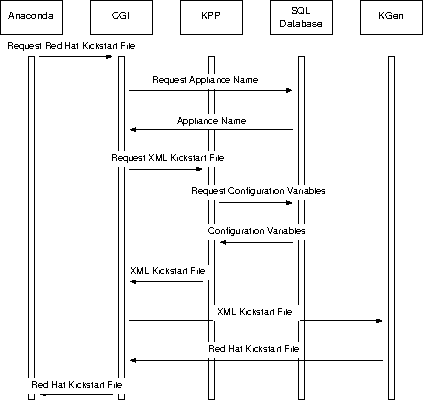
\includegraphics[width=0.8\textwidth,height=0.7\textwidth]
		{pics/alurkickstart.pdf}
	\caption{Alur Perjalanan \f{Kickstart}}
	\label{fig:alurkickstart}
\end{figure}
\begin{center}
{\small Sumber gambar: \citep{paper.jackson}}
\end{center}

Kata-kata dalam gambarnya bisa di hover, magic!!

%-----------------------------------------------------------------------------%
\subsection{Rocks Rolls}
%-----------------------------------------------------------------------------%
Untuk contoh konten Rolls dapat dilihat pada gambar \ref{fig:contohisiroll}. Pada contoh tersebut, \f{package} yang mengandung konfigurasi \f{graph} adalah berkas \co{roll-sge-kickstart-3.2.0-0.noarch.rpm} \citep{paper.jackson}. 


\begin{figure}
	\centering
	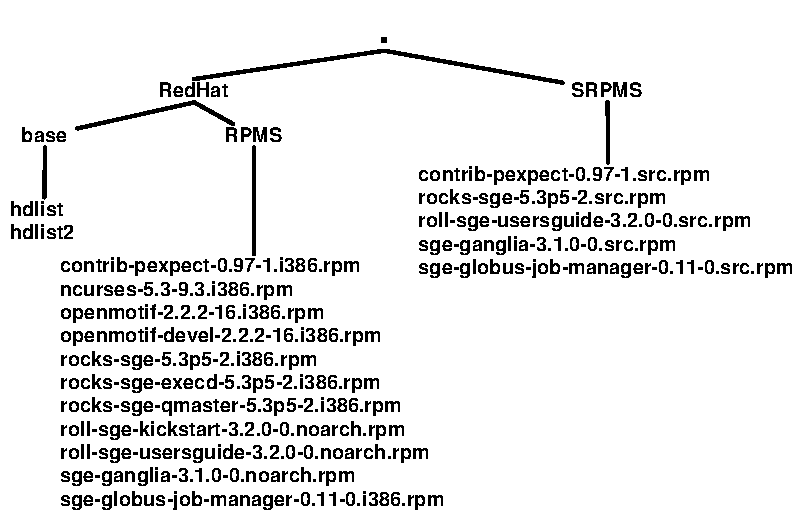
\includegraphics[width=0.9\textwidth,height=0.6\textwidth]
		{pics/rollexample.pdf}
	\caption{Contoh konten yang berada dalam \f{Rolls}}
	\label{fig:contohisiroll}
\end{figure}
\begin{center}
{\small Sumber gambar: \citep{paper.jackson}}
\end{center}

COde-like words : \code{FIRSTFIT} atau \code{BESTFIT} \citep{paper.jackson}. 

%-----------------------------------------------------------------------------%
\section{Mengubah Tampilan Teks}
%-----------------------------------------------------------------------------%
Beberapa perintah yang dapat digunakan untuk mengubah tampilan adalah: 
\begin{itemize}
	\item \bslash f \\
		Merupakan alias untuk perintah \bslash textit, contoh 
		\f{contoh hasil tulisan}.
	\item \bslash bi \\
		\bi{Contoh hasil tulisan}.
	\item \bslash bo \\
		\bo{Contoh hasil tulisan}.
	\item \bslash code \\ 
		\code{Contoh hasil tulisan}.
\end{itemize}


%-----------------------------------------------------------------------------%
\section{Memberikan Catatan}
%-----------------------------------------------------------------------------%
Ada dua perintah untuk memberikan catatan penulisan dalam dokumen yang Anda 
kerjakan, yaitu: 
\begin{itemize}
	\item \bslash todo \\
		Contoh: \\ \todo{Contoh bentuk todo.}
	\item \bslash todoCite \\ 
		Contoh: \todoCite
\end{itemize}


%-----------------------------------------------------------------------------%
\section{Menambah Isi Daftar Isi}
%-----------------------------------------------------------------------------%
Terkadang ada kebutuhan untuk memasukan kata-kata tertentu kedalam Daftar Isi. 
Perintah \bslash addChapter dapat digunakan untuk judul bab dalam Daftar isi. 
Contohnya dapat dilihat pada berkas thesis.tex.
%-----------------------------------------------------------------------------%
\chapter{\babEmpat}
%-----------------------------------------------------------------------------%
%-----------------------------------------------------------------------------%
\section{Membuat Tabel}
%-----------------------------------------------------------------------------%
Seperti pada gambar, tabel juga dapat diberi label dan caption. 
Caption pada tabel terletak pada bagian atas tabel. 
Contoh tabel sederhana dapat dilihat pada \tab~\ref{tab:tab1}.

\begin{table}
	\centering
	\caption{Contoh Tabel}
	\label{tab:tab1}
	\begin{tabular}{| l | c r |}
		\hline
		& kol 1 & kol 2 \\ 
		\hline
		baris 1 & 1 & 2 \\
		baris 2 & 3 & 4 \\
		baris 3 & 5 & 6 \\
		jumlah  & 9 & 12 \\
		\hline
	\end{tabular}
\end{table}

Ada jenis tabel lain yang dapat dibuat dengan \latex~berikut 
beberapa diantaranya. 
Contoh-contoh ini bersumber dari 
\url{http://en.wikibooks.org/wiki/LaTeX/Tables}

\begin{table}
	\centering
	\caption{An Example of Rows Spanning Multiple Columns}
	\label{row.spanning}
	\begin{tabular}{|l|l|*{6}{c|}}
  		\hline % create horizontal line
  		No & Name & \multicolumn{3}{|c|}{Week 1} & \multicolumn{3}{|c|}{Week 2} \\
  		\cline{3-8} % create line from 3rd column till 8th column
  		& & A & B & C & A & B & C\\
  		\hline
  		1 & Lala & 1 & 2 & 3 & 4 & 5 & 6\\
  		2 & Lili & 1 & 2 & 3 & 4 & 5 & 6\\
  		3 & Lulu & 1 & 2 & 3 & 4 & 5 & 6\\
  		\hline
	\end{tabular}
\end{table}

\begin{table}
	\centering
	\caption{An Example of Columns Spanning Multiple Rows}
	\label{column.spanning}
	\begin{tabular}{|l|c|l|}
		\hline
		Percobaan & Iterasi & Waktu \\
		\hline
		Pertama & 1 & 0.1 sec \\ \hline
		\multirow{2}{*}{Kedua} & 1 & 0.1 sec \\
 		& 3 & 0.15 sec \\ 
 		\hline
		\multirow{3}{*}{Ketiga} & 1 & 0.09 sec \\
 		& 2 & 0.16 sec \\
 		& 3 & 0.21 sec \\ 
 		\hline
	\end{tabular}
\end{table}

\begin{table}
	\centering
	\caption{An Example of Spanning in Both Directions Simultaneously}
	\label{mix.spanning}
	\begin{tabular}{cc|c|c|c|c|}
		\cline{3-6}
		& & \multicolumn{4}{|c|}{Title} \\ \cline{3-6}
		& & A & B & C & D \\ \hline
		\multicolumn{1}{|c|}{\multirow{2}{*}{Type}} &
		\multicolumn{1}{|c|}{X} & 1 & 2 & 3 & 4\\ \cline{2-6}
		\multicolumn{1}{|c|}{}                        &
		\multicolumn{1}{|c|}{Y} & 0.5 & 1.0 & 1.5 & 2.0\\ \cline{1-6}
		\multicolumn{1}{|c|}{\multirow{2}{*}{Resource}} &
		\multicolumn{1}{|c|}{I} & 10 & 20 & 30 & 40\\ \cline{2-6}
		\multicolumn{1}{|c|}{}                        &
		\multicolumn{1}{|c|}{J} & 5 & 10 & 15 & 20\\ \cline{1-6}
	\end{tabular}
\end{table}

%-----------------------------------------------------------------------------%
\section{thesis.tex}
%-----------------------------------------------------------------------------%
Berkas ini berisi seluruh berkas Latex yang dibaca, jadi bisa dikatakan sebagai 
berkas utama. Dari berkas ini kita dapat mengatur bab apa saja yang ingin 
kita tampilkan dalam dokumen.


%-----------------------------------------------------------------------------%
\section{laporan\_setting.tex}
%-----------------------------------------------------------------------------%
Berkas ini berguna untuk mempermudah pembuatan beberapa template standar. 
Anda diminta untuk menuliskan judul laporan, nama, npm, dan hal-hal lain yang 
dibutuhkan untuk pembuatan template. 


%-----------------------------------------------------------------------------%
\section{istilah.tex}
%-----------------------------------------------------------------------------%
Berkas istilah digunakan untuk mencatat istilah-istilah yang digunakan. 
Fungsinya hanya untuk memudahkan penulisan.
Pada beberapa kasus, ada kata-kata yang harus selalu muncul dengan tercetak 
miring atau tercetak tebal. 
Dengan menjadikan kata-kata tersebut sebagai sebuah perintah \latex~tentu akan 
mempercepat dan mempermudah pengerjaan laporan. 


%-----------------------------------------------------------------------------%
\section{hype.indonesia.tex}
%-----------------------------------------------------------------------------%
Berkas ini berisi cara pemenggalan beberapa kata dalam bahasa Indonesia. 
\latex~memiliki algoritma untuk memenggal kata-kata sendiri, namun untuk 
beberapa kasus algoritma ini memenggal dengan cara yang salah. 
Untuk memperbaiki pemenggalan yang salah inilah cara pemenggalan yang benar 
ditulis dalam berkas hype.indonesia.tex.
%-----------------------------------------------------------------------------%
\chapter{\babLima}
%-----------------------------------------------------------------------------%

%-----------------------------------------------------------------------------%
\section{Implementasi \f{Cluster}}
%-----------------------------------------------------------------------------%

%-----------------------------------------------------------------------------%
\subsection{Instalasi \f{Frontend}}
%-----------------------------------------------------------------------------%
Tabel model lain, ditunjukkan pada tabel \ref{tab:infohasti}. 
\begin{table}
	\centering
	\caption{Informasi \f{cluster} X}
	\newcolumntype{g}{>{\columncolor{headertbl}}c}
	\label{tab:infohasti}
	\begin{tabular}{|g|c|}
	\hline Host Name & X\\
	\hline Cluster Name & X\\
	\hline Certificate Organization & UI\\
	\hline Certificate Locality & Depok\\
	\hline Certificate State & West Java\\
	\hline Certificate Country & ID\\
	\hline Contact & X\\
	\hline URL & http://grid.ui.ac.id\\
	\hline
	\end{tabular}
\end{table}

Ada pagebreak disini.
%supaya rapih
\pagebreak

Another type of table
\begin{table}
	\centering
	\caption{Perbandingan Partisi \f{default} dan manual}
	\newcolumntype{g}{>{\columncolor{headertbl}}c}
	\label{tab:partdisk}
	\begin{tabular}{|g|c|c|}
	\rowcolor{headertbl}
	\hline & Partisi default & Partisi manual yang dilakukan\\
	\hline / & 16 GB & 30 GB\\
	\hline /var & 4 GB & 18 GB\\
	\hline swap & 1 GB & 2 GB\\
	\hline /export & 55 GB & 26 GB\\
	\hline
	\end{tabular}
\end{table}

Program menghasilkan keluaran seperti pada kode \ref{lst:raidready}. 

\begin{minipage}{\linewidth}
\begin{lstlisting}[caption={Keluaran output},label={lst:raidready}]
[root@nas-0-0 ~]# cat /proc/mdstat 
Personalities : [raid1] 
md0 : active raid1 sda4[0] sdb2[1]
      1917672312 blocks super 1.2 [2/2] [UU]
      
unused devices: <none>
[root@nas-0-0 ~]# mdadm --detail /dev/md0 
/dev/md0:
        Version : 1.2
  Creation Time : Fri May  3 15:38:52 2013
     Raid Level : raid1
     Array Size : 1917672312 (1828.83 GiB 1963.70 GB)
  Used Dev Size : 1917672312 (1828.83 GiB 1963.70 GB)
   Raid Devices : 2
  Total Devices : 2
    Persistence : Superblock is persistent

    Update Time : Tue May 28 11:27:49 2013
          State : clean 
 Active Devices : 2
Working Devices : 2
 Failed Devices : 0
  Spare Devices : 0

           Name : nas-0-0.local:0  (local to host nas-0-0.local)
           UUID : 0754726d:3dfbd4b9:42b0f587:68631556
         Events : 28

    Number   Major   Minor   RaidDevice State
       0       8        4        0      active sync   /dev/sda4
       1       8       18        1      active sync   /dev/sdb2
\end{lstlisting}
\end{minipage}

%-----------------------------------------------------------------------------%
\subsection{Konfigurasi}\label{cha:confcluster}
%-----------------------------------------------------------------------------%
Contoh verbatim dalam itemize : 
\begin{itemize}
\item \bo{Bold ini}\\
dijalankan perintah berikut : 
\begin{Verbatim}[frame=single]
# javac Ganteng.java
# java Ganteng
\end{Verbatim}
\paragraph{}
Perilaku sistem 
\begin{Verbatim}[frame=single]
# hai
# enable
# cd /export/rocks/install/
# create distro
# sh sesuatu.sh
# reboot
\end{Verbatim}
\paragraph{}

\item \bo{Menambahkan \f{package} pada \f{compute node}}\\
Langkah yang dilakukan adalah sebagai berikut : 
	\begin{enumerate}
	\item Masuk ke dalam direktori \co{/procfs/}
	\item Membuat/Mengubah berkas \co{xx.xml}. Jika tidak terdapat berkas tersebut, dapat disalin dari \co{skeleton.xml}.
	\item Menambahkan \f{package} yang ingin dipasang pada \f{compute node} diantara \f{tag} \co{<package>} seperti berikut : \co{<package>[package yang akan dipasang]</package>}.
	\item Menjalankan perintah berikut termasuk perintah untuk melakukan instalasi ulang seluruh \f{compute node}: 
	\begin{Verbatim}[frame=single]
# cd /export/somedir
# create
# run host
	\end{Verbatim}
	\end{enumerate}
	\paragraph{}
\end{itemize}
%-----------------------------------------------------------------------------%
\subsubsection{semakin ke dalam}
%-----------------------------------------------------------------------------%
\begin{minipage}{\linewidth}
\begin{lstlisting}[caption={Keluaran mentah untuk detail \f{job}}, label={lst:outqstatf},style=L]
[ardhi@xx ~]$ qstat -f 138
Job Id: 138.xx
    Job_Name = cur-1000-1np
    Job_Owner = ardhi@xx
    resources_used.cput = 27:21:35
    resources_used.mem = 86060kb
    resources_used.vmem = 170440kb
    resources_used.walltime = 27:24:50
    job_state = R
    queue = default
    server = hastinapura.grid.ui.ac.id
    Checkpoint = u
    ctime = Fri May 31 10:27:37 2013
    Error_Path = xx:/home/ardhi/xx/curcumin-1000/cur-1000-1np.e138
    exec_host = compute-0-5/0
    exec_port = 15003
    Hold_Types = n
    Join_Path = n
    Keep_Files = n
    Mail_Points = e
    Mail_Users = ardhi.putra@ui.ac.id
    mtime = Fri May 31 10:27:47 2013
    Output_Path = xx:/home/ardhi/xx/curcumin-1000/cur-1000-1np.o138
    Priority = 0
    qtime = Fri May 31 10:27:37 2013
    Rerunable = True
    Resource_List.nodes = 1:ppn=1
    session_id = 5768
    etime = Fri May 31 10:27:37 2013
    submit_args = cur-1000-1np.pbs
    start_time = Fri May 31 10:27:47 2013
    submit_host = xx
    init_work_dir = /home/ardhi/xx/curcumin-1000   
\end{lstlisting}
\end{minipage}

%-----------------------------------------------------------------------------%
\section{Pengujian} %lebih ke gimana cara ujinya
%-----------------------------------------------------------------------------%

%-----------------------------------------------------------------------------%
\subsection{Kasus Uji}
%-----------------------------------------------------------------------------%
Berwarna!
\begin{lstlisting}[caption=Potongan skrip submisi \f{job} melalui torqace,label={lst:grotorqace},style=shell]
# Go To working directory
cd $PBS_O_WORKDIR

#openMPI prerequisite
. /opt/torque/etc/openmpi-setup.sh

mpirun -np 5 -machinefile $PBS_NODEFILE mdrun -v -s \ 
	curcum400ps.tpr -o md_prod_curcum400_5np.trr -c lox_pr.gro
...
\end{lstlisting}
%-----------------------------------------------------------------------------%
\subsection{Kasus Uji}
%-----------------------------------------------------------------------------%
Contoh skrip yang dimasukkan pada \f{form} yang disediakan dapat dilihat pada kode \ref{lst:makebzip}.
\begin{lstlisting}[caption={Potongan \co{Makefile} \f{project}}, label={lst:makebzip},style=shell]
# Make file for MPI
SHELL=/bin/sh

# Compiler to use
# You may need to change CC to something like CC=mpiCC
# openmpi : mpiCC
# mpich2  : /opt/mpich2/gnu/bin/mpicxx
CC=mpiCC
...
...
\end{lstlisting}
%-----------------------------------------------------------------------------%
\chapter{\babEnam}
%-----------------------------------------------------------------------------%

%-----------------------------------------------------------------------------%
\section{Hasil Pengujian}
%-----------------------------------------------------------------------------%
%-----------------------------------------------------------------------------%
\subsection{Hasil Pengujian Kasus Uji 1}
%-----------------------------------------------------------------------------%
Tabel lain. Hasil tersebut dapat dilihat pada tabel \ref{tab:hasilgrrd}.
\begin{table}
	\centering
	\caption{Hasil pengujian menggunakan gromacs}
	\label{tab:hasilgrrd}
	\begin{tabular}{|c|l|*{3}{c|}}
		\rowcolor{headertbl}
  		\hline % create horizontal line
  		No & \f{Timestep} & \multicolumn{3}{|>{\columncolor{headertbl}}c|}{Waktu eksekusi berdasar jumlah prosesor} \\
		\hhline{|>{\arrayrulecolor{headertbl}}*{2}{-}>{\arrayrulecolor{black}}*{3}{|-|}}
  		\rowcolor{headertbl} & & 1 & 2 & 5 \\
  		\hline 1 & 200ps & 20h:27m:16s & 12h:59m:04s & 5h:07m:03s \\
  		\hline 2 & 400ps & 1d:22h:40m:03s & 1d:02h:08m:47s & 10h:09m:39s \\
  		\hline 3 & 600ps & 2d:23h:29m:21s & 1d:14h:52m:52s & 15h:25m:22s \\
  		\hline 4 & 800ps & 4d:02h:05m:57s & 2d:03h:30m:07s & 20h:29m:38s \\
  		\hline 5 & 1000ps & 5d:03h:29m:12s & 2d:16h:32m:22s & 1d:01h:34m:38s \\
  		\hline
	\end{tabular}
\end{table}
%-----------------------------------------------------------------------------%
\section{Evaluasi Hasil Kasus Uji}
%-----------------------------------------------------------------------------%
%-----------------------------------------------------------------------------%
\subsection{Evaluasi Kasus Uji 1}
%-----------------------------------------------------------------------------%
Tabel \ref{tab:hasilgrrd} menunjukkan hasil uji coba pada penelitian ini.  Gambar \ref{fig:grafgro5} menunjukkan perbandingan waktu eksekusi pada aplikasi x dengan jumlah prosesor sebanyak 5 buah.

\begin{figure}
	\centering
	\includegraphics[width=1\textwidth]
		{pics/5np-gromacs-chart.pdf}
	\caption{Perbandingan waktu eksekusi x untuk 5 prosesor}
	\label{fig:grafgro5}
\end{figure}
\paragraph{}
%-----------------------------------------------------------------------------%
\chapter{\babTujuh}
%-----------------------------------------------------------------------------%
Pada bab terakhir ini, 
%---------------------------------------------------------------
\section{Kesimpulan}
%---------------------------------------------------------------

%---------------------------------------------------------------
\section{Saran}
%---------------------------------------------------------------


%\printbibliography
%
% Daftar Pustaka
%\include{pustaka}
%biblama (bukan biblatex)
\bibliography{bib}{}
%\bibliography{references}{}
%biblama (bukan biblatex)
\bibliographystyle{apalikerd}
%\bibliographystyle{ieeetr} 

%
% Lampiran 
%
\begin{appendix}
	%
% @author  Andreas Febrian
% @version 1.00 
% 
% Hanya sebuah pembatas bertuliskan LAMPIRAN ditengah halaman. 
% 

\begin{titlepage}
	\centering 
	\vspace*{6cm}
	\noindent \Huge{LAMPIRAN}
	\addChapter{LAMPIRAN}
\end{titlepage}
	\setcounter{page}{2}
	%-----------------------------------------------------------------------------%
\addChapter{Lampiran 1 : Kode Sumber}
\chapter*{Lampiran 1 : Kode Sumber}
%-----------------------------------------------------------------------------%
\section*{\code{admin\_useraddmaster}} \label{cha:lampir-admin}
Skrip ini diletakkan pada direktori \co{/usr/sesuatu} dan hanya dapat dieksekusi oleh \f{root}. Skrip ini berguna untuk menambahkan pengguna baru sesuai dengan konfigurasi baru yang telah ditetapkan.
\begin{lstlisting}[style=L,caption={Skrip menambahkan pengguna baru},label={lst:adduser}]
#!/bin/csh -f
blah blah blah
blah blah blah
blah blah blah
blah blah blah
blah blah blah
\end{lstlisting}

\section*{\code{getuser.cron}} \label{cha:lampir-cronadmin}
Penjelasan skrip disini
\begin{lstlisting}[style=L,caption={\f{Cronjob} menambahkan pengguna baru},label={lst:cronadduser}]
#!/bin/bash
# Change these two lines to localize to your system:
# Adapted from /usr/local/sbin/admin_useradd

cat /dev/null > $userlist
for (( i=0; i<${#listemailto[@]}; i++ ))
do
        uname=${listusername[$i]}
        mailto=${listemailto[$i]}

        echo "User $uname created, please use torqace wisely." | mail -s "Torqace user registration" $mailto
done

\end{lstlisting}

%-----------------------------------------------------------------------------%
\addChapter{Lampiran 2 : Berkas Konfigurasi}
\chapter*{Lampiran 2 : Berkas Konfigurasi}
%-----------------------------------------------------------------------------%
\section*{compute.xml}
\begin{lstlisting}[caption={Berkas \co{compute.xml}},label={lst:excomp},language=XML]
<?xml version="1.0" standalone="no"?>
<kickstart>
<description>
	Compute node XML file
</description>
</kickstart> 
\end{lstlisting}

%-----------------------------------------------------------------------------%
\addChapter{Lampiran 8 : UAT dan Kuesioner}
%-----------------------------------------------------------------------------%
\begin{landscape}
\chapter*{Lampiran 8 : UAT dan Kuesioner}
\begin{longtable}{|c|p{7cm}|p{2.5cm}|p{3.5cm}|p{3.3cm}|p{1.8cm}|}
\caption{Tabel UAT dan Kuesioner} \label{tab:uattbl}\\
\hline
No. & \multicolumn{1}{c|}{Langkah Penggunaan} & Fitur Berjalan & Tingkat Kemudahan (1-5) & Tingkat Kepuasan (1-5) & Saran / Komentar \\ 
\cline{3-5} & & Berhasil /Tidak & 1:Sangat sulit ; \hspace{100pt} 5:sangat mudah & 1 : Sangat kecewa ; 5 : sangat puas &  \\ \hline
\multicolumn{ 6}{|>{\columncolor{headertbl}}c|}{Use Case : Login} \\ \hline
1.1 & Pengguna berada pada halaman depan torqace &  &  &  &  \\ \hline
1.2 & Pengguna memasukkan username dan password pada field yang telah disediakan.Kemudian menekan tombol 'login' &  &  &  &  \\ \hline
1.3 & Apabila Sukses, maka pengguna masuk ke dalam sistem dan dihadapkan pada menu utama &  &  &  &  \\ \hline
\multicolumn{ 6}{|>{\columncolor{headertbl}}c|}{Use Case : Register} \\ \hline
2.1 & Pengguna berada pada halaman registrasi pengguna torqace &  &  &  &  \\ \hline
2.2 & Pengguna memasukkan username,password, dan email pada field yang telah disediakan. Kemudian menekan tombol 'submit' &  &  &  &  \\ \hline
2.3 & Sistem akan mengonfirmasi masukan, dan akan mengirimkan email untuk memberitahu pengguna apabila proses pendaftaran telah selesai &  &  &  &  \\ \hline
\multicolumn{ 6}{|>{\columncolor{headertbl}}c|}{Use Case : Logout} \\ \hline
3.1 & Pengguna memilih menu untuk melakukan logout &  &  &  &  \\ \hline
3.2 & Sistem akan mengeluarkan pengguna, dan pengguna tidak dapat menggunakan fitur-fitur utama aplikasi &  &  &  &  \\ \hline
\multicolumn{ 6}{|>{\columncolor{headertbl}}c|}{Use Case : Upload Job Sederhana} \\ \hline
4.1 & Pengguna memilih menu upload file/project pada menu utama &  &  &  &  \\ \hline
4.2 & Pengguna memilih pilihan 'single file' pada tipe project &  &  &  &  \\ \hline
4.3 & Pengguna memilih berkas yang akan diunggah, mengisi label, dan menentukan apakah akan menimpa project sebelumnya dengan nama yang sama atau tidak &  &  &  &  \\ \hline
4.4 & Pengguna menekan tombol 'submit' dan mengonfirmasi  &  &  &  &  \\ \hline
4.5 & Sistem akan menampilkan informasi terkait berkas yang diupload &  &  &  &  \\ \hline
\multicolumn{ 6}{|>{\columncolor{headertbl}}c|}{Use Case : Upload Job Compressed} \\ \hline
5.1 & Pengguna memilih menu upload file/project pada menu utama &  &  &  &  \\ \hline
5.2 & Pengguna memilih pilihan 'compressed files' pada tipe project &  &  &  &  \\ \hline
5.3 & Pengguna memilih arsip yang akan diunggah, mengisi label, menentukan akan melakukan make atau tidak dan menentukan apakah akan menimpa project sebelumnya dengan nama yang sama atau tidak &  &  &  &  \\ \hline
5.4 & Pengguna menekan tombol 'submit' dan mengonfirmasi  &  &  &  &  \\ \hline
5.5 & Sistem akan menampilkan informasi terkait berkas yang diupload dan diekstrak. Keluaran make juga akan ditampilkan bila dipilih &  &  &  &  \\ \hline
\multicolumn{ 6}{|>{\columncolor{headertbl}}c|}{Use Case : Upload Array Job} \\ \hline
6.1 & Pengguna memilih menu upload file/project pada menu utama &  &  &  &  \\ \hline
6.2 & Pengguna memilih pilihan 'array' pada tipe project &  &  &  &  \\ \hline
6.3 & Pengguna memilih arsip-arsip yang akan diunggah, mengisi label, menentukan akan melakukan make atau tidak dan menentukan apakah akan menimpa project sebelumnya dengan nama yang sama atau tidak &  &  &  &  \\ \hline
6.4 & Pengguna menekan tombol 'submit' dan mengonfirmasi  &  &  &  &  \\ \hline
6.5 & Sistem akan menampilkan informasi terkait berkas yang diupload dan diekstrak. Keluaran make juga akan ditampilkan bila dipilih &  &  &  &  \\ \hline
\multicolumn{ 6}{|>{\columncolor{headertbl}}c|}{Use Case : Melihat antrian pada queue} \\ \hline
7.1 & Pengguna memilih menu  queue status pada menu utama &  &  &  &  \\ \hline
7.2 & Pengguna berada pada halaman yang berisi informasi queue &  &  &  &  \\ \hline
\multicolumn{ 6}{|>{\columncolor{headertbl}}c|}{Use Case : Melihat detil antrian} \\ \hline
8.1 & Dari halaman status queue, pengguna memilih job tertentu &  &  &  &  \\ \hline
8.2 & Informasi mengenai detil job tersebut ditampilkan dalam bentuk tabel &  &  &  &  \\ \hline
8.2.1 & Apabila job tersebut bukan milik pengguna, maka sistem akan melarang pengguna melihat informasi detil suatu job &  &  &  &  \\ \hline
\multicolumn{ 6}{|>{\columncolor{headertbl}}c|}{Use Case : Membuat script job} \\ \hline
9.1 & Pengguna memilih untuk melakukan 'generate script' baik dari laporan upload berkas, atau dari penjelajahan direktori &  &  &  &  \\ \hline
9.2 & Pengguna mengisi nama job, parameter job, dan script yang akan dijalankan.  &  &  &  &  \\ \hline
9.3 & Pengguna mengonfirmasi konfirmasi submit job &  &  &  &  \\ \hline
9.4 & Pengguna dapat melihat informasi script secara keseluruhan dan pesan apakah terjadi kegagalan atau tidak, serta id job yang diberikan &  &  &  &  \\ \hline
\multicolumn{ 6}{|>{\columncolor{headertbl}}c|}{Use Case : Load spesifikasi job lain} \\ \hline
10.1 & Pengguna berada pada halaman untuk membuat script &  &  &  &  \\ \hline
10.2 & Pengguna memilih 'Load a Previous Job' &  &  &  &  \\ \hline
10.3 & Pengguna memilih job mana yang akan dimuat dan menekan tombol 'Load' &  &  &  &  \\ \hline
10.4 & Pengguna kembali ke halaman pembuatan script dengan spesifikasi job sebelumnya &  &  &  &  \\ \hline
\multicolumn{ 6}{|>{\columncolor{headertbl}}c|}{Use Case : Menjelajah Direktori} \\ \hline
11.1 & Pengguna memilih menu  'View File/Project'  pada menu utama &  &  &  &  \\ \hline
11.2 & Pengguna dapat melakukan navigasi untuk masuk ke dalam direktori tertentu, atau kembali ke direktori diatasnya, dan dapat melihat terdapat berkas apa saja dalam direktori &  &  &  &  \\ \hline
\multicolumn{ 6}{|>{\columncolor{headertbl}}c|}{Use Case : Menghapus Berkas/Direktori} \\ \hline
12.1 & Pengguna berada pada halaman penjelajahan direktori &  &  &  &  \\ \hline
12.2 & Pengguna memilih pilihan untuk menghapus berkas/direktori di samping item yang akan dihapus &  &  &  &  \\ \hline
12.3 & Pengguna mengonfirmasi konfirmasi penghapusan &  &  &  &  \\ \hline
\multicolumn{ 6}{|>{\columncolor{headertbl}}c|}{Use Case : Mengunduh Berkas/Direktori} \\ \hline
13.1 & Pengguna berada pada halaman penjelajahan direktori &  &  &  &  \\ \hline
13.2 & Pengguna memilih pilihan untuk mengunduh berkas/direktori di samping item yang akan dihapus &  &  &  &  \\ \hline
\multicolumn{ 6}{|>{\columncolor{headertbl}}c|}{Use Case : Melihat Berkas} \\ \hline
14.1 & Pengguna berada pada halaman penjelajahan direktori &  &  &  &  \\ \hline
14.2 & Pengguna memilih berkas yang berupa berkas teks &  &  &  &  \\ \hline
14.3 & Sistem akan menampilkan konten dari berkas tersebut &  &  &  &  \\ \hline
\end{longtable}
\end{landscape}
\end{appendix}

\end{document}